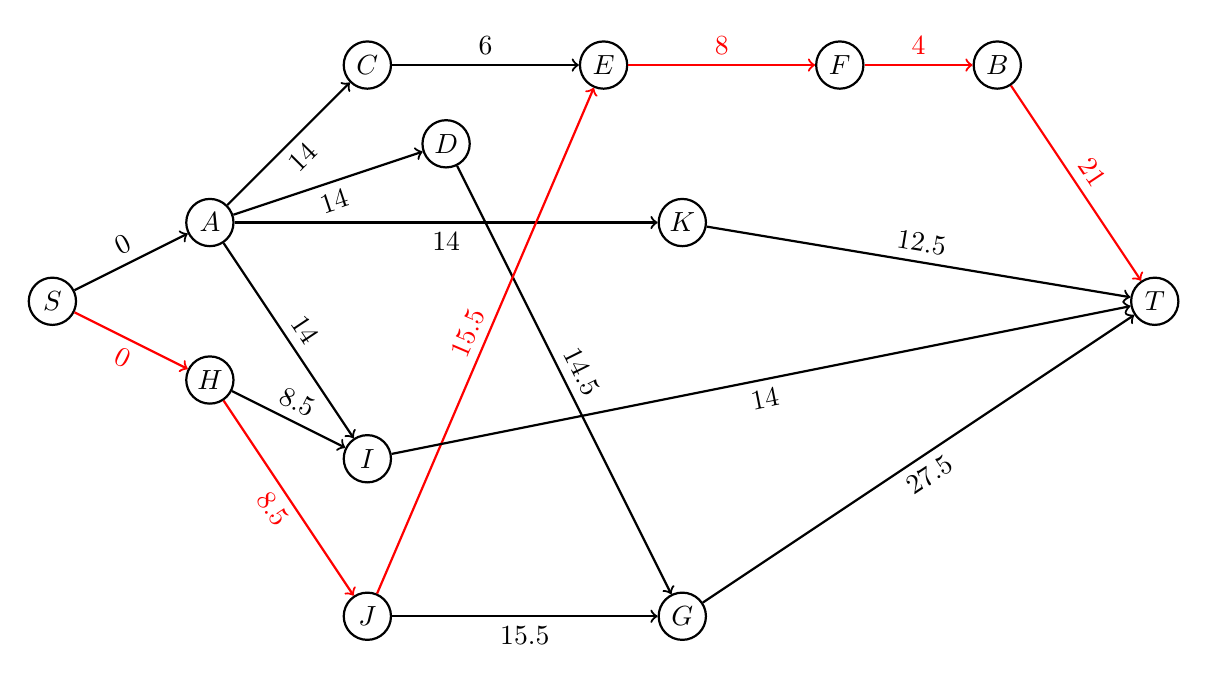
\begin{tikzpicture}[style=thick,scale=1]
\tikzstyle{every node}=[]
\tikzstyle{vertex}=[draw, circle, fill=white, inner sep=0pt, minimum size=6mm]

\node[vertex] (S) at (-6, 0) {$S$};
\node[vertex] (A) at (-4, 1) {$A$};
\node[vertex] (B) at (6, 3) {$B$};
\node[vertex] (C) at (-2, 3) {$C$};
\node[vertex] (D) at (-1, 2) {$D$};
\node[vertex] (E) at (1, 3) {$E$};
\node[vertex] (F) at (4, 3) {$F$};
\node[vertex] (G) at (2, -4) {$G$};
\node[vertex] (H) at (-4, -1) {$H$};
\node[vertex] (I) at (-2, -2) {$I$};
\node[vertex] (J) at (-2, -4) {$J$};
\node[vertex] (K) at (2, 1) {$K$};
\node[vertex] (T) at (8, 0) {$T$};

\draw[->,red] (S) -- (H) node[midway, below, sloped] {$0$};
\draw[->] (S) -- (A) node[midway, above, sloped] {$0$};
\draw[->] (A) -- (C) node[midway, below, sloped] {$14$};
\draw[->] (A) -- (D) node[midway, below, sloped] {$14$};
\draw[->] (A) -- (K) node[midway, below, sloped] {$14$};
\draw[->] (A) -- (I) node[midway, above, sloped] {$14$};
\draw[->,red] (H) -- (J) node[midway, below, sloped] {$8.5$};
\draw[->] (H) -- (I) node[midway, above, sloped] {$8.5$};
\draw[->] (D) -- (G) node[midway, above, sloped] {$14.5$};
\draw[->] (J) -- (G) node[midway, below, sloped] {$15.5$};
\draw[->,red] (J) -- (E) node[midway, above, sloped] {$15.5$};
\draw[->] (C) -- (E) node[midway, above, sloped] {$6$};
\draw[->] (I) -- (T) node[midway, below, sloped] {$14$};
\draw[->] (K) -- (T) node[midway, above, sloped] {$12.5$};
\draw[->,red] (E) -- (F) node[midway, above, sloped] {$8$};
\draw[->] (G) -- (T) node[midway, below, sloped] {$27.5$};
\draw[->,red] (F) -- (B) node[midway, above, sloped] {$4$};
\draw[->,red] (B) -- (T) node[midway, above, sloped] {$21$};

\end{tikzpicture}